\section{Il database}

Una definizione di database può essere presa da Wikipedia [Wikipedia] {\bf il database rappresenta un archivio di dati strutturati}; la struttura più diffusa in questo momento è quella chiamata \emph{relazionale}, che si compone di tabelle e di relazioni tra di esse.

\subsection{Database Prolog}
Il database sarà una teoria prolog, dove le tabelle verranno espresse come una lista di fatti (\emph{facts}) dove ogni atomo della lista rappresenterà una riga di tale tabella. Il nome della tabella sarà il predicato mentre gli argomenti saranno i valori delle colonne. Per rappresentare una tabella di nome nomeTabella con N colonne (col1...colN) potrò usare la seguente sintassi:
\begin{lstlisting}[language=Prolog]
 nomeTabella(col1,col2,......,colN).
\end{lstlisting}
Un caso particolare può essere: 
\begin{lstlisting}[language=Prolog]
 tabella(col1,col2,col3).
 tabella(col1,col2).
\end{lstlisting}
questi due termini sono ambigui, non si sa cosa si voglia rappresentare; potrebbe essere che la col3 è null e quindi è stata omessa? oppure la seconda tabella è una tabella diversa dalla prima? per semplificare ho retenuto che nel caso si presenti una situazione del genere venga generata un'eccezione e si lasci all'utente decidere come disambinguare la situazione. Un modo per risolvere potrebbe essere quello usare il termine \emph{null} come valore, esempio : 

\begin{lstlisting}[language=Prolog]
 ta(col1,col2,col3).
 ta(col1,null,col2).
\end{lstlisting} 

Il termine \emph{null} ovviamente dovrà essere minuscolo altrimenti dal prolog verrebbe considerato una variabile. 

\subsubsection{Tipi di dato e Strutture dati}
Il database così costruito ha come tipi di dati primitivi gli stessi supportati dal prolog; come strutture dati supporta gli Array in quanto sono facilmente rappresentabili in prolog come delle liste. 

\subsection{Il metabase}
Per avere la completezza di informazioni tipiche di un moderno database relazionale è necessario avere delle ulteriori informazioni su come è strutturato il database ed in particolare sulla struttura delle tabelle; queste informazioni solitamente compongono quello che è chiamato \emph{metabase} o \emph{metadatabase}. Un possibile insieme di informazioni utili possono essere : 
\begin{enumerate}
\item il nome da associare ad una colonna
\item il tipo di dato che contiene una colonna
\item la descrizione del contenuto di una colonna 
\end{enumerate}
questi sono solo alcuni possibili elementi. Nel nostro caso il \emph{metabase} può essere descritto attraverso l'uso di una tabella di sistema dal nome {\bf mtable}; la sintassi sarà : 
\begin{lstlisting}[language=Prolog,showstringspaces=false]
 mtable(
	"nome tabella",
	"posizione della colonna tra gli argomenti",
	"nome della colonna",
	"tipo di dato contenuto",
 ).
\end{lstlisting}
Questa particolare tabella non è pero necessaria, il database sarà comuque consistente, ma la sua presenza facilita l'interazione dell'utente nello scrivere query sql. Un esempio :
\begin{lstlisting}[language=Prolog,showstringspaces=false]
 mtable("ta",1,"colonna1","string").
\end{lstlisting}
Permetterà all'utente di usare il nome della colonna nelle clausole sql.

\subsection{Store Procedure e Function}
E' possibile pensare a far supportare al database prolog anche le \emph{store procedure} e le \emph{function}  in quanto in una teoria prolog oltre ai fatti si possono inserire anche delle regole (\emph{rules}). Il supporto a tale funzionalità è stato rimandato a estensioni future. 

\subsection{Struttura}

Dal punto di vista strutturale il database è stato cosi strutturato : 
\begin{itemize}
\item[-] Catalog : è il contenitore di schema
\item[-] Schema : è quello che viene chiamato impropriamente database 
\item[-] Table : è la tabella canonca
\end{itemize}

Sul filesystem il catalog è visto come una cartella, al cui interno ci sono gli schema sottoforma di file con l'estensione .db;  invece per i database di sistema è riservato l'uso dell'estensione .dbs  (Es. metabase.dbs) la cui presenza è però facoltativa. Il nome del database è il nome del file senza l'estensione, questo per ragioni di semplicità, mentre il nome del catalog è il nome della directory. L'utilizzo del catalog si è resa necessaria per poter , in futuro, dare supporto a query sql multi-schema, cosa ormai diffusa nell'uso di un database relazionale. 

\begin{figure}[ht]
\centering
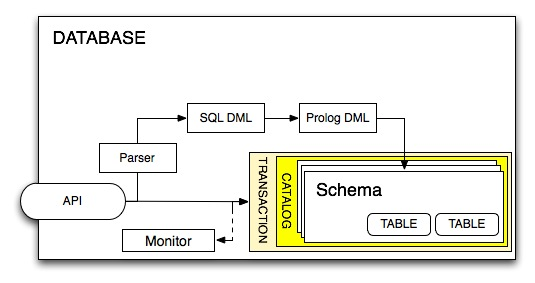
\includegraphics[width=1\textwidth]{immagini/struttura.jpg}
\caption{Database Structure}\label{fig:immagini/struttura.jpg}
\end{figure}
